\chapter{Założenia projektowe}
\label{chap:zalozenia-projektowe}
\section{Wymagania funkcjonalne}
\label{sec:wymagania-funkcjonalne}

%Na razie do wglądu diagramy use cases
% Jest kilka kwestii do dyskusji
% W systemie powinny być kategorie usera i rodziny. User moze edytowac swoje kategorie a admin rodziny rodzinne kategorie. Gdy konto jest dodane do rodziny mozna mu dodawac kategorie rodziny ale tez usera
% 1 pytanie czy use case diagram dla category jest poprawny (generalizacja) Moze powinny byc osobne use casy dla kategorii rodziny i osobne dla kategorii usera

%2 family use case: czy admin powinien moc nadawac uprawnienia do nieswojego konta? Cz powinien admin moze domyslnie i zawsze dodawac wydatki do nieswojego konta, czy moze wlasciciel musi mu nadac uprawninia. 

\begin{figure}[p]
	\centering
	\fbox{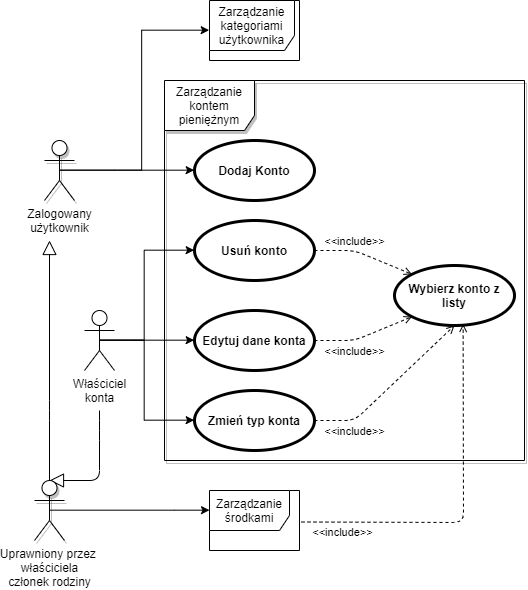
\includegraphics[width=.6\linewidth]{rys03/use-case-account.png}}
	\caption{Diagram przypadków użycia konta pieniężnego}
	\label{fig:use-case-account}
\end{figure}

\begin{figure}[p]
	\centering
	\fbox{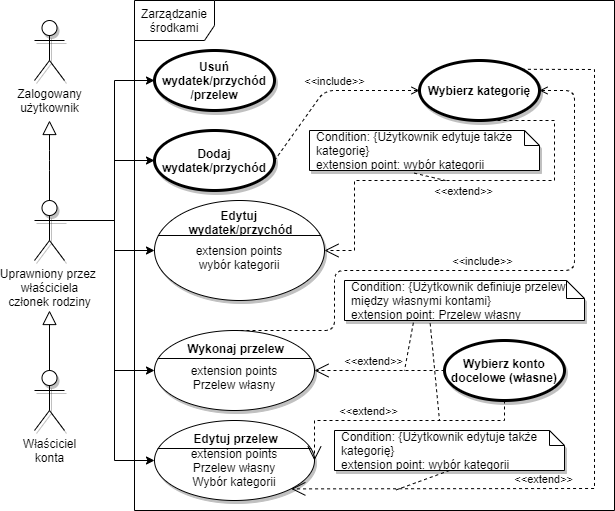
\includegraphics[width=.6\linewidth]{rys03/use-case-money.png}}
	\caption{Subdiagram przypadków użycia dla operacji finansowych}
	\label{fig:use-case-money}
\end{figure}

\begin{figure}[p]
	\centering
	\fbox{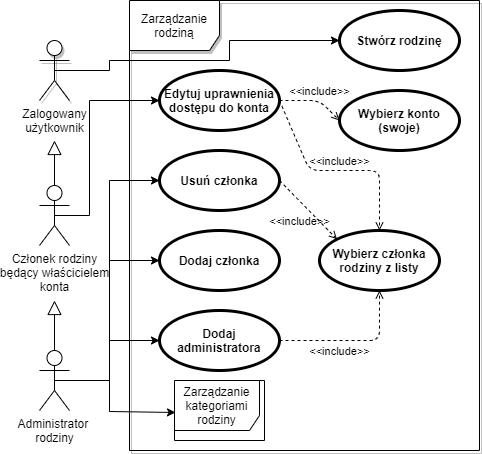
\includegraphics[width=.6\linewidth]{rys03/use-case-family.png}}
	\caption{Diagram przypadków użycia dla kategorii}
	\label{fig:use-case-category}
\end{figure}

\begin{figure}[p]
	\centering
	\fbox{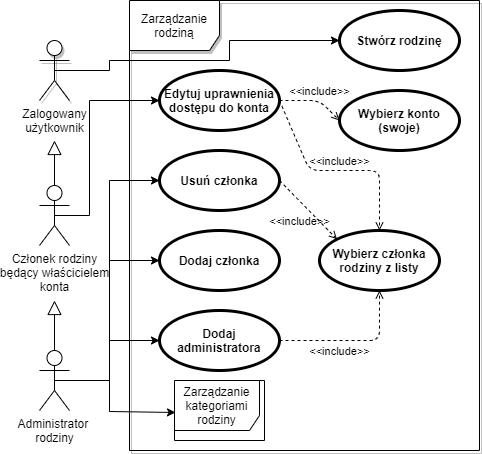
\includegraphics[width=.6\linewidth]{rys03/use-case-family.png}}
	\caption{Diagram przypadków użycia dla rodziny}
	\label{fig:use-case-family}
\end{figure}


\section{Wymagania niefunkcjonalne}
\label{sec:wymagania-niefunkcjonalne}

\begin{enumerate}[labelwidth=\widthof{\ref{last-item}},label=\arabic*.]

\item System składać ma się z~dwóch głównych części:
\begin{enumerate}[label=\alph*)]
\item aplikacji serwerowej -- API. Jej zadaniem będzie dostarczanie interfejsu programistycznego do pobierania danych i~modyfikowania stanu systemu.
\item aplikacja webowej, dostarczająca graficzny interfejs użytkownika -- \texttt{GUI}. Aplikacja ta będzie konsumować API.
\end{enumerate}

\item Zarówno aplikacja webowa, jak i API będą stworzone przy pomocy frameworka ASP.NET Core w wersji co najmniej 2.2: 
\begin{enumerate}[label=\alph*)]
\item Do napisania aplikacji webowej użyte zostaną \texttt{Razor Pages} oraz komponenty widoku (ang.~\emph{view components}). 
\item Warstwa persystencji danych w aplikacji API stworzona zostanie z pomocą Entity Framework Core 2.2. Wykorzystane zostanie podejście \emph{code first} i mechanizm migracji.
\end{enumerate}

\item Pobieranie danych z API ma odbywać się za pomocą protokołu OData.

\item API używać będzie bazy danych na serwerze Microsoft SQL Server 2017 (lub nowszym).

\item Aplikacja webowa powinna poprawnie działać co najmniej w przeglądarkach: Mozilla Firefox, Google Chrome, Opera, Microsoft Edge oraz Safari, a~także przeglądarkach mobilnych: Opera Mobile, Google Chrome, Mozilla Firefox i Safari.

\item Aplikacja będzie wymuszać działanie z wykorzystaniem protokołu \texttt{HTTPS} (ang.~\emph{Hypertext Transfer Protocol Secure}).

\item Autoryzacja i uwierzytelnienie ma być przeprowadzona z wykorzystaniem protokołu OpenId Connect i frameworka autoryzacji OAuth 2.0. Użyty powinien zostać \emph{Hybrid Flow} lub \emph{Authorization Code Flow}.

\item Dostawcą tożsamości w systemie powinna być osobna aplikacja, posiadająca własną bazę danych lub zewnętrzy system autoryzacji, np.~\texttt{Auth0}.

\item API ma posiadać dokumentację stworzoną przy pomocy narzędzia \texttt{Swagger}.

\item Kod źródłowy ma być napisany z wykorzystaniem dobrych praktyk programowania~i~wzorców projektowych ułatwiających jego utrzymanie i rozwijanie.

\item System działać będzie na platformie chmurowej \texttt{Microsfot Azure}.

\item Poszczególne składowe systemu w chmurze powinny być automatycznie skalowalne.

\item Aplikacja webowa powinna być bezpieczna i odporna na ataki. Zostanie wykorzystany mechanizm obrony przed \texttt{CSRF} (ang.~Cross-Site Request Forgery) -- \texttt{anti-forgery token}.

\end{enumerate}

\section{Metodyka}
\label{sec:metodyka}













\begin{figure}[b]
\setlayoutscale{0.43}
\currentstock
\oddpagelayouttrue
\twocolumnlayoutfalse
\drawmarginparstrue
\drawparametersfalse
\drawstock
\caption{Rzeczywisty układ strony nieparzystej w tym dokumencie} \label{fig:currentPageLayout}
\end{figure}







\begin{figure}[b]
	\centering
	\fbox{
\includegraphics[width=.6\linewidth]{rys03/praca-dyplomowa2}}
	\caption{Oficjalny szablon strony tytułowej pracy dyplomowej, \url{http://www.logotyp.pwr.edu.pl/Default.aspx?page=PracaDyplomowa} [dostęp dnia 20.04.2016]}
	\label{fig:stronaTytulowa}
\end{figure}

\begin{table}[htb]
\centering
\caption{Zestawienie czcionek elementów podziału dokumentu, tekstu wiodącego, nagłówka i stopki oraz podpisów (Rozm. -- rozmiar czcionki, Odst. -- \texttt{baselineskip})}
\label{tab:secfonts}\small
\begin{tabularx}{\linewidth}{|ll@{\hskip 5pt}l@{\hskip 5pt}lX|} \hline
Element & Przykład & Czcionka & Rozm. & Odst. \\ \hline\hline
Nr rozdziału & {\huge\bfseries Rozdział 1 } & \verb?\huge\bfseries? & 25pt & 30pt \\
Tytuł rozdziału & {\Huge\bfseries Wstęp } & \verb?\Huge\bfseries? & 30pt & 37pt\\
Nr i tytuł sekcji & {\Large\bfseries 1.1. Wprowadzenie } & \verb?\Large\bfseries? & 17pt & 22pt \\
Nr i tytuł podsekcji & {\large\bfseries 1.1.1. Cel szczegółowy } & \verb?\large\bfseries? &14.5pt & 18pt\\
Tytuł podpodsekcji  & {\normalsize\bfseries Założenia } & \verb?\normalsize\bfseries? & 12pt & 14.5pt\\
Tytuł paragrafu & {\normalsize\bfseries  Podstawy } Opis ... &  \verb?\normalsize\bfseries? & 12pt & 14.5pt\\
Tekst wiodący & {\normalsize Niniejszy dokument ... } & \verb?\normalsize? & 12pt & 14.5pt\\
Nagłówek strony & {\small\itshape 3.2. Czcionka wiodąca ...} & \verb?\small\itshape? & 11pt & 13.6pt \\
Stopka strony & {\small Imię Nazwisko: ...} & \verb?\small? & 11pt & 13.6pt\\
Podpisy tabel & {\small Tab.~3.1: Zestawienie ...} & \verb?\small? & 11pt & 13.6pt \\
Podpisy rysunków & {\small Rys.~3.1: Oficjalny ...} & \verb?\small? & 11pt & 13.6pt\\\hline
\end{tabularx}
\end{table}
